% !TeX program = xelatex
% !TeX encoding = UTF-8
% !TeX spellcheck = en_US
% !BIB program = biber
%% 
%%%%%%%%%%%%%%%%%%%%%%%%%%%%%%%%%%%%%%%%%%%%%%%%%%%%%%%%%%%%%%%%%%%%%%%%%%%%%%%%

%%%%%%%%%%%%%%%%%%%%%%%%%%%%%%%%%%%%%%%%%%%%%%%%%%%%%%%%%%%%%%%%%%%%%%%%%%%%%%%%
%% 
%%            JJJJ   K                         K   UUUU         UUUU  
%%            JJJJ   KKKK                   KKKK   UUUU         UUUU  
%%            JJJJ   KKKKKK               KKKKKK   UUUU         UUUU  
%%            JJJJ      KKKKKK         KKKKKK      UUUU         UUUU  
%%            JJJJ         KKKKKK   KKKKKK         UUUU         UUUU  
%%            JJJJ            KKKKKKKKK            UUUU         UUUU  
%%    JJ     JJJJJ               KKK               UUUUU       UUUUU  
%%  JJJJJJJJJJJJJ    KKKKKKKKKKKKKKKKKKKKKKKKKKK    UUUUUUUUUUUUUUU   
%%    JJJJJJJJJ      KKKKKKKKKKKKKKKKKKKKKKKKKKK      UUUUUUUUUUU     
%% 
%% This is an example file for using the JKU LaTeX technical report template
%% for your technical report.
%% 
%% Template created by Michael Roland (2021)
%% 
%%%%%%%%%%%%%%%%%%%%%%%%%%%%%%%%%%%%%%%%%%%%%%%%%%%%%%%%%%%%%%%%%%%%%%%%%%%%%%%%

%%%%%%%%%%%%%%%%%%%%%%%%%%%%%%%%%%%%%%%%%%%%%%%%%%%%%%%%%%%%%%%%%%%%%%%%%%%%%%%%
%% 
\documentclass[a4paper,oneside,10pt,ngerman]{scrartcl}
\usepackage[utf8]{inputenc}
\usepackage[
    TNF,
    equalmargins,
    techreport,
    nofancyfonts,
    logopath=../logos,
    fontpath=../fonts
]{../jkureport}
%% 
%%%%%%%%%%%%%%%%%%%%%%%%%%%%%%%%%%%%%%%%%%%%%%%%%%%%%%%%%%%%%%%%%%%%%%%%%%%%%%%%

%%%%%%%%%%%%%%%%%%%%%%%%%%%%%%%%%%%%%%%%%%%%%%%%%%%%%%%%%%%%%%%%%%%%%%%%%%%%%%%%
%% 
\usepackage{enumerate}
\usepackage{listingsutf8}
\usepackage{graphicx}
\usepackage{siunitx}
%% 
%%%%%%%%%%%%%%%%%%%%%%%%%%%%%%%%%%%%%%%%%%%%%%%%%%%%%%%%%%%%%%%%%%%%%%%%%%%%%%%%

\newcommand{\designspath}{../../designs}
\graphicspath{{images/}}
\newcolumntype{Y}{>{\centering\arraybackslash}X}

\begin{document}
%%%%%%%%%%%%%%%%%%%%%%%%%%%%%%%%%%%%%%%%%%%%%%%%%%%%%%%%%%%%%%%%%%%%%%%%%%%%%%%%
%% 
%% Report information and title page
%% 

\title{Single-Ended OPV}

\subtitle{UE - Technische Elektronik \\%
    \usekomafont{subtitlesmall}%
    \hfill\\%
    SoSe24\\
    \hfill\\%
}

\author{%
    Simon Grundner
    \affiliation{Institute for Integrated Circuits}
    \authornewline
    \authormail{k12136610@students.jku.at}
    \authorweb{https://jku.at/iic}
    \authornewline
}

\partnerlogo{../logos/iic}
\reportnumber{Aufgabe 2}
\setbottommark{Simon Grundner, k12136610}
\keywords{MOSFETs, Differenzenverstärker, CMRR, OSIC-Tools}

\maketitle
%% 
%%%%%%%%%%%%%%%%%%%%%%%%%%%%%%%%%%%%%%%%%%%%%%%%%%%%%%%%%%%%%%%%%%%%%%%%%%%%%%%%

\tableofcontents

%%%%%%%%%%%%%%%%%%%%%%%%%%%%%%%%%%%%%%%%%%%%%%%%%%%%%%%%%%%%%%%%%%%%%%%%%%%%%%%%
%% 
\newpage
\section{Single-Ended OPV}

\begin{highlightblock}[Aufgabe: Single-Ended OPV]
    Zu Analysieren ist ein Single-Ended OPV, welcher aus einem
    Differenzverstärker und einer Ausgangsstufe besteht. Analysen beinhalten DC
    Sweeps, AC Analyses und Berechnungen zur Gleichtaktunterdrückung. Die $W/L$
    Verhältnisse der MOSFETs sind so zu wählen, dass eine große Verstärkung und
    großes CMRR erreicht wird.
\end{highlightblock}

\subsection{Schaltung}

\begin{figure}[h]
    \centering
    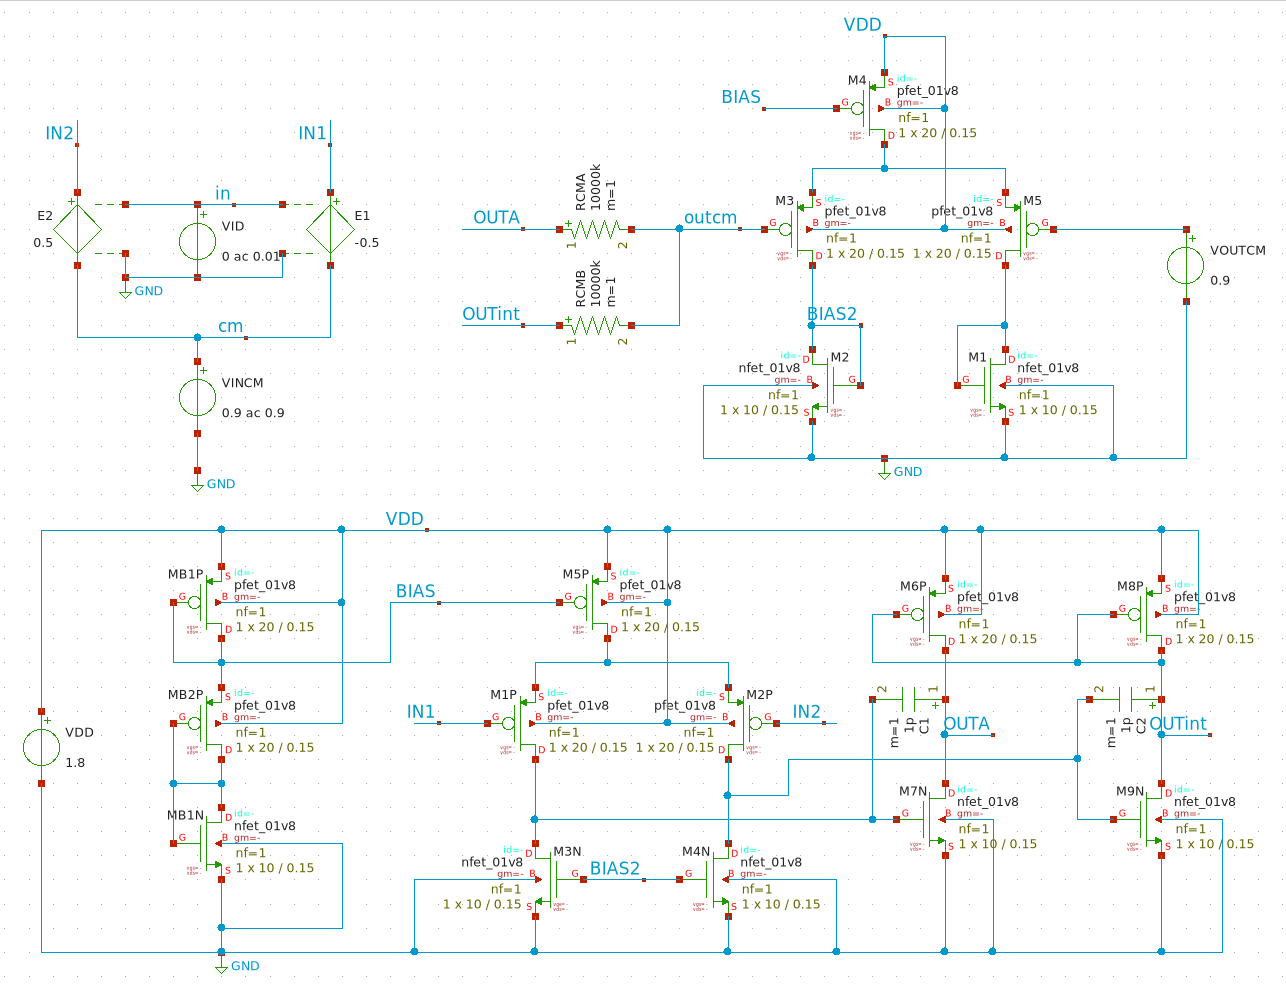
\includegraphics[width=.9\textwidth]{schem.png}
    \caption{Single-Ended OPV Schaltung}\label{fig:schem}
\end{figure}

\newpage
\subsection{Simulation ohne W/L Anpassung}

Zunächst wurde die Schaltung mit den Standard W/L Verhältnissen simuliert, um
Vergleichswerte zu erhalten.

\begin{itemize}
    \item $W/L = 20/0.15 \frac{\si{\nano\meter}}{\si{\nano\meter}}$
\end{itemize}

\subsubsection{DC Sweep}

\lstinputlisting[
    firstline=444,
    lastline=456
]{\designspath/Aufgabe2_k12136610.sch}

\textbf{Ein- und Ausgangsverhältnisse}

Für den Differenzeneingang wurde $V_{ID}$ von \SI{-200}{\milli\volt} bis
\SI{0}{\milli\volt} Simuliert. Für die Gleichtakteingang wurde
$V_{CM}=\SI{900}{\milli\volt}$ fest eingestellt. In \autoref{fig:1-dc-diff}
ist das Ergebnis des DC Sweeps für den Gegentakteingang zu sehen und in
\autoref{fig:1-dc-cm} das Ergebnis für den Gleichtakteingang. Die Labels sind
im Schaltplan in \autoref{fig:schem} zu finden.

Hier ist zu erkennen, dass der Gegentakteingang für kleine Signale bereits
standardmäßig um einen höheren Faktor verstärkt wird als der Gleichtakteingang.
Ab etwa \SI{-100}{\milli\volt} Befindet sich der Ausgang bereits in sättigung.

\begin{figure}[h]
\begin{minipage}{.45\textwidth}
    \centering
    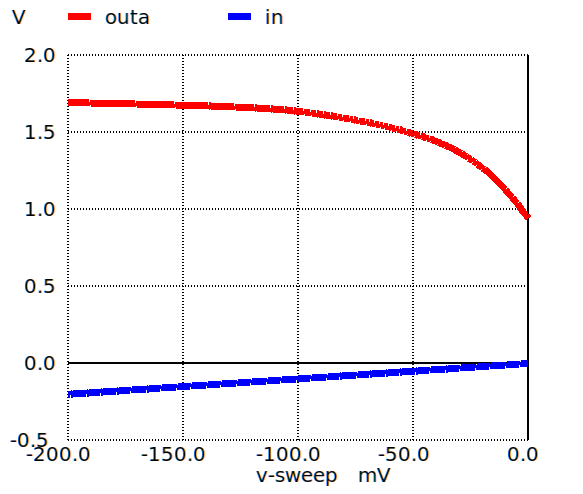
\includegraphics[height=5cm]{1-dc-diff.png}
    \caption{DC Sweep Differenzeingang}\label{fig:1-dc-diff}
\end{minipage}\hfill
\begin{minipage}{.45\textwidth}
    \centering
    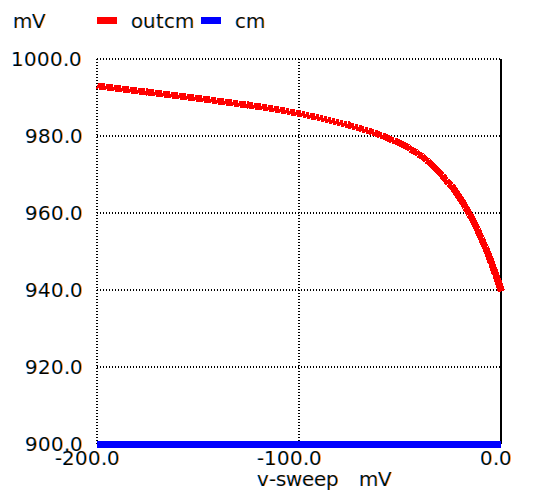
\includegraphics[height=5cm]{1-dc-cm.png}
    \caption{DC Sweep Gleichtakt}\label{fig:1-dc-cm}
\end{minipage}
\end{figure}

\newpage
\textbf{Gleichtakt- und Gegentaktverstärkung}

In \autoref{fig:1-dc-a} sind die Verstärkungen für Gleich- und Gegentakt
dargestellt. In \autoref{fig:1-dc-cmrr} ist das daraus resultierende
Gleichtaktunterdrückungsverhältnis (CMRR) in dezibel angegeben.

\begin{figure}[h]
\begin{minipage}{.45\textwidth}
    \centering
    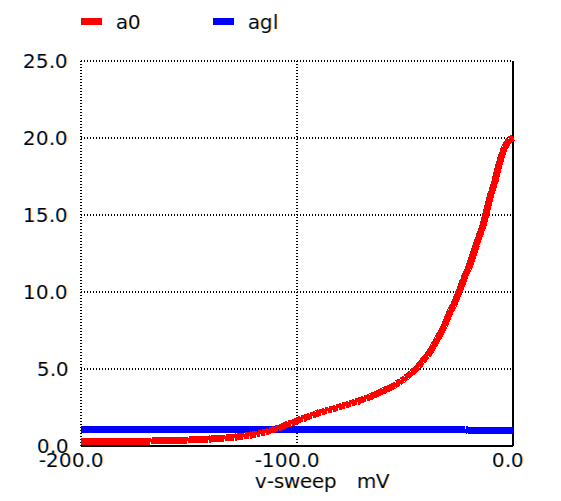
\includegraphics[height=5cm]{1-dc-a.png}
    \caption{Gleich- und Gegentaktverstärkung}\label{fig:1-dc-a}
\end{minipage}\hfill
\begin{minipage}{.45\textwidth}
    \centering
    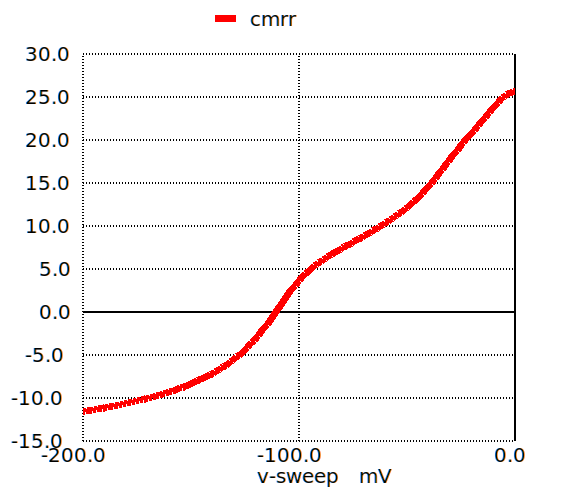
\includegraphics[height=5cm]{1-dc-cmrr.png}
    \caption{CMRR}\label{fig:1-dc-cmrr}
\end{minipage}
\end{figure}

Die Verstärkung ist aufgrund der invertierenden PMOS Eingangstufe nahe Null maximal. Je höher
die Eingangsspannung, desto kleiner wird die Gegentaktverstärkung, bis sie
schließlich die Gleichtaktverstärkung unterschreitet. In
\autoref{fig:1-dc-cmrr} ist zu erkennen, dass dann das CMRR negativ wird. 

\begin{table}[h]
    \caption{Maximal Verstärkungswerte ohne W/L Anpassung}
    \begin{tabularx}{\textwidth}{XX}
        Gegentaktverstärkung $A_0$ & Gleichtaktverstärkung $A_{CM}$ \\ \midrule
        \num{20.1} & \num{1.1} \\
    \end{tabularx}
\end{table}

\subsubsection{AC Analyse}

Ähnlich wie bei der DC Analyse werden hier die gleichen Parameter untersucht.

\lstinputlisting[
    firstline=463,
    lastline=473
]{\designspath/Aufgabe2_k12136610.sch}

\newpage

\textbf{Ein- und Ausgangsverhältnisse}

\begin{figure}[h]
\begin{minipage}{.45\textwidth}
    \centering
    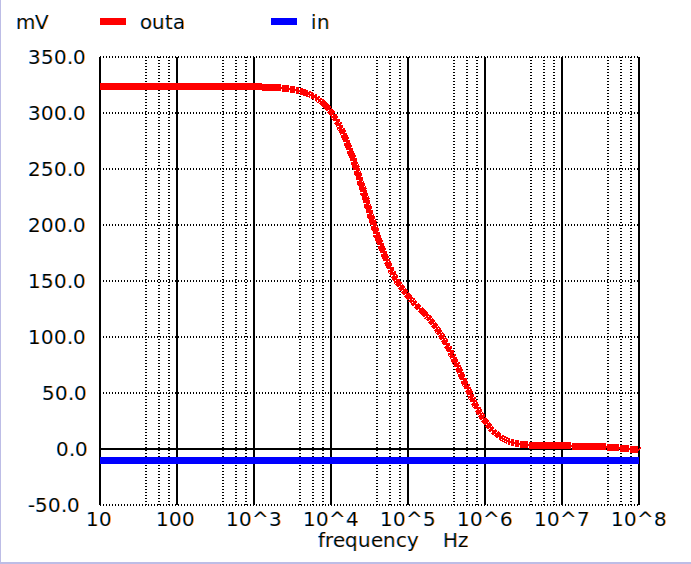
\includegraphics[height=5cm]{1-ac-diff.png}
    \caption{AC Analyse Differenzeingang}\label{fig:1-ac-diff}
\end{minipage}\hfill
\begin{minipage}{.45\textwidth}
    \centering
    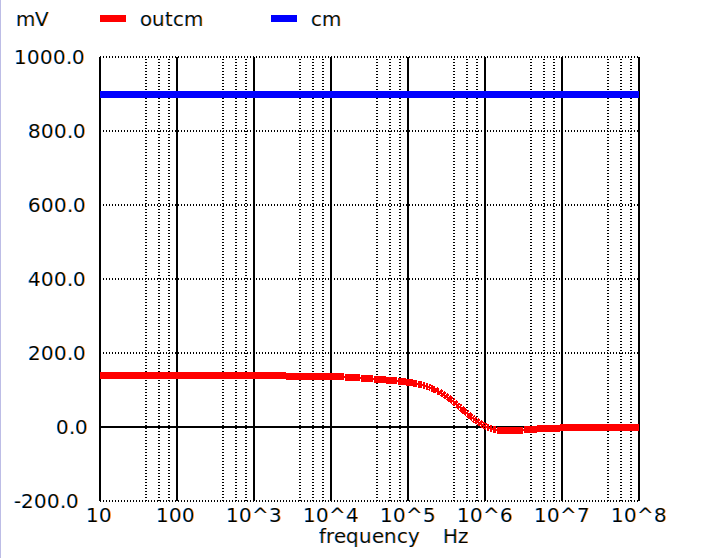
\includegraphics[height=5cm]{1-ac-cm.png}
    \caption{AC Analyse Gleichtakt}\label{fig:1-ac-cm}
\end{minipage}
\end{figure}

\textbf{Gleichtakt- und Gegentaktverstärkung}

\begin{figure}[h]
\begin{minipage}{.32\textwidth}
    \centering
    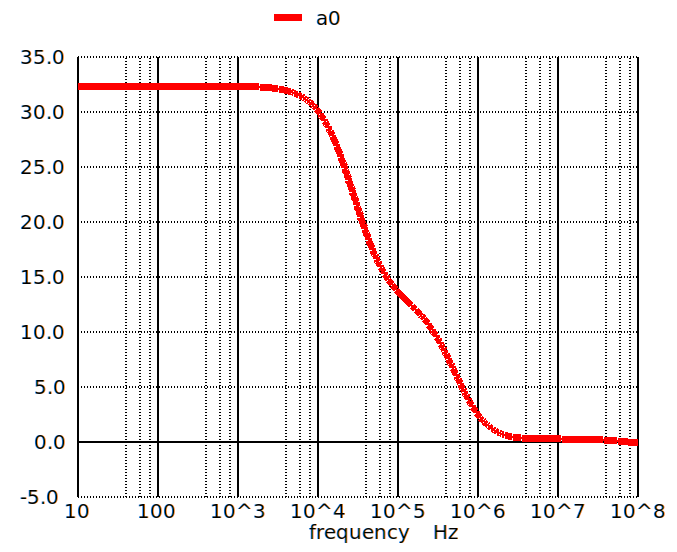
\includegraphics[width=\textwidth]{1-ac-a0.png}
    \caption{$A_0$}\label{fig:1-ac-a0}
\end{minipage}\hfill
\begin{minipage}{.32\textwidth}
    \centering
    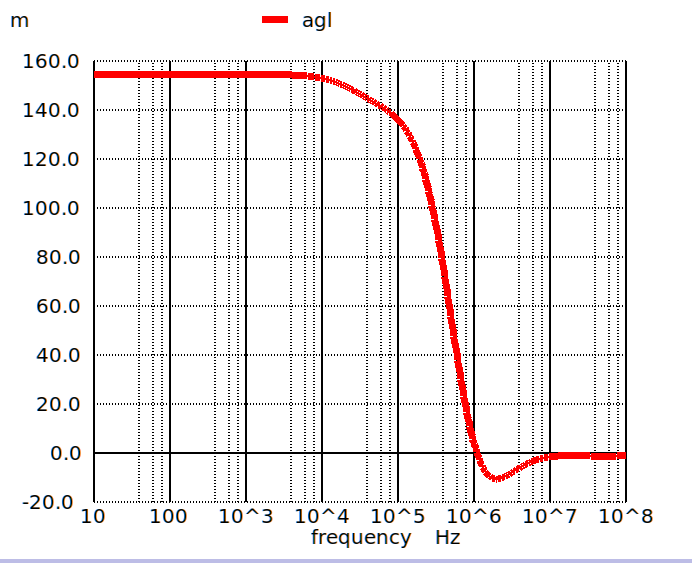
\includegraphics[width=\textwidth]{1-ac-agl.png}
    \caption{$A_{gl}$}\label{fig:1-ac-agl}
\end{minipage}\hfill
\begin{minipage}{.32\textwidth}
    \centering
    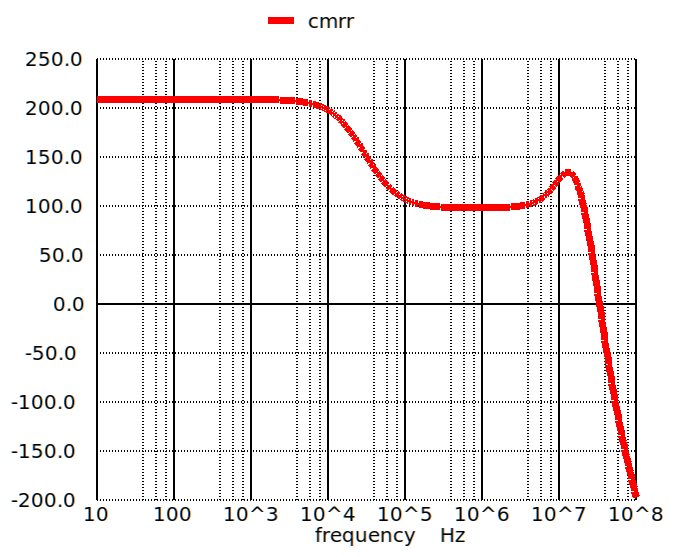
\includegraphics[width=\textwidth]{1-ac-cmrr.png}
    \caption{$CMRR$}\label{fig:1-ac-cmrr}
\end{minipage}
\end{figure}

\subsection{Simulation mit W/L Anpassung}

Ziel ist es die Verstärkung $A_0 = -g_m\cdot R_{out}$ zu erhöhen, indem
$R_{out}$ und $g_m$ maximiert werden.

Um $g_m$ und $R_0$ zu erhöhen werden folgende zusammenhänge berücksichtigt:

\begin{itemize}
    \item $g_m = \dfrac{I_D}{n U_T}$ im schwachen Inversionsbereich
    \item $g_m = \dfrac{I_D}{U_{gs}-U_{th}}$ im starken Inversionsbereich
    \item $g_m \propto \dfrac{W}{L}$
    \item $R_{out} \propto L$
\end{itemize}

Die Anhaltspunkte sind nun $W/L$ und $L$ zu erhöhen. Um den Strom $I_D$ zu
erhöhen, kann die Biasspannung näher an $V_{DD}$ gelegt werden.

Ziel ist es auch die Gleichtaktverstärkung zu verringern. Dazu soll bei
$V_{ID}=0$ und $V_{INCM}= 0.9V$ die Gleichtaktspannung am Ausgang dem
Designziel $V_{OUTCM}=0.9$ Entsprechen.

\newpage
\subsubsection{Optimierung 1: Gatelängen der Ausgangsstufe erhöhen}

Um den Ausgangswiderstand zu erhöhen, wurden die Gatelängen der Transistoren
M6-M9 Verdoppelt. Das W/L Verhältnis bleibt dabei unverändert. Hier lassen sich
bereits verbesserungen der Differenzenverstärkung erkennen bei einer
unveränderten Gleichtaktspannung. Demzufolge trotzdem ein verbessertes CMRR.

\begin{figure}[h]
\begin{minipage}{.32\textwidth}
    \centering
    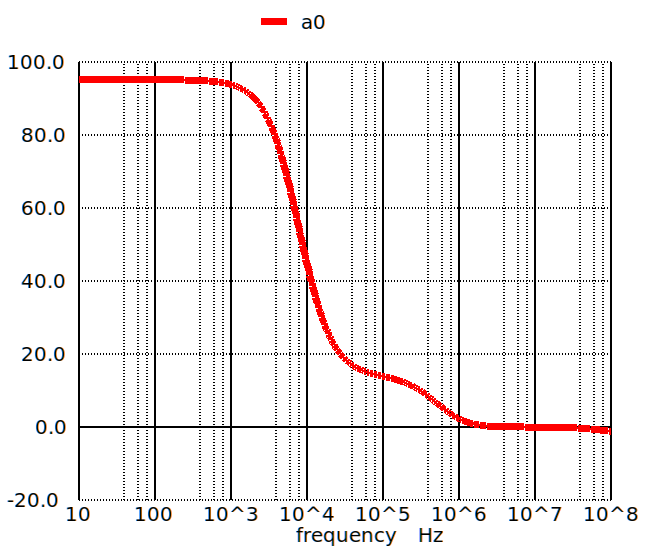
\includegraphics[width=\textwidth]{2-ac-a0.png}
    \caption{$A_0$}\label{fig:2-ac-a0}
\end{minipage}\hfill
\begin{minipage}{.32\textwidth}
    \centering
    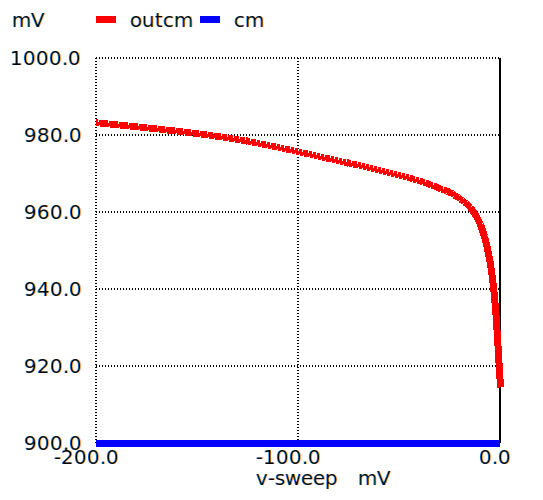
\includegraphics[width=\textwidth]{2-dc-cm.png}
    \caption{CM Ein und Ausgang}\label{fig:2-dc-cm}
\end{minipage}\hfill
\begin{minipage}{.32\textwidth}
    \centering
    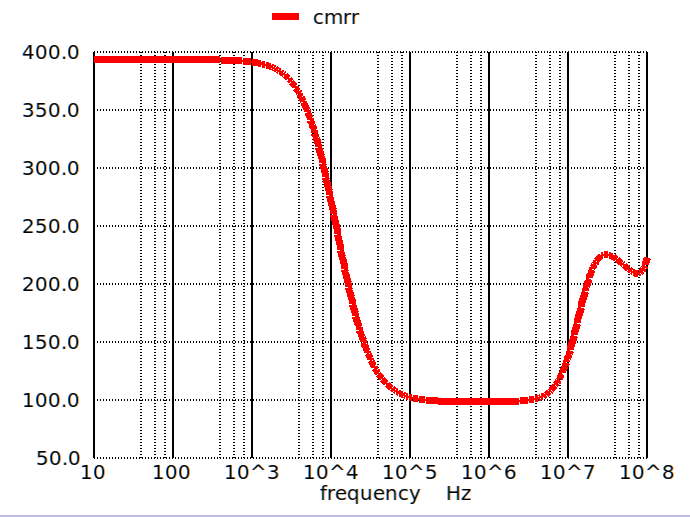
\includegraphics[width=\textwidth]{2-ac-cmrr.png}
    \caption{$CMRR$}\label{fig:2-ac-cmrr}
\end{minipage}
\end{figure}

Das Ziel von $V_{OUTCM}=0.9V$ wurde jedoch noch nicht erreicht.

\subsubsection{Optimierung 2: Differenzeneingansstufe anpassen}

An der Eingangsstufe wurde der Querstrom erhöht, indem die Gatelängen der
Transistoren die den Stromspiegel Ausmachen erhöht wurden. Durch den erhöhten
Querstrom wurde auch $W$ für ein höheres $g_m$ angepasst.

\begin{itemize}
    \item PMOST M5: $W/L = 40/0.15$
    \item NMOST M3, M4: $W/L = 40/0.16$
\end{itemize}

Auch das W/L Verhältnis der Eingangstransistoren wurde erhöht:

\begin{itemize}
    \item PMOST M1, M2: $W/L = 40/0.2$
\end{itemize}

\newpage
\subsubsection{DC Sweep}

$OUTCM$ konnte durch die Anpassungen auf \SI{0.892}{\volt} gebracht werden, wie
in \autoref{fig:3-dc-cm} zu sehen ist und auch in der Simulation ausgegeben
wird. Auch die ausgangsverstärkung wurde durch die Anpassung der Eingangsstufe stark erhöht.

\begin{figure}[h]
    \begin{minipage}{.45\textwidth}
        \centering
        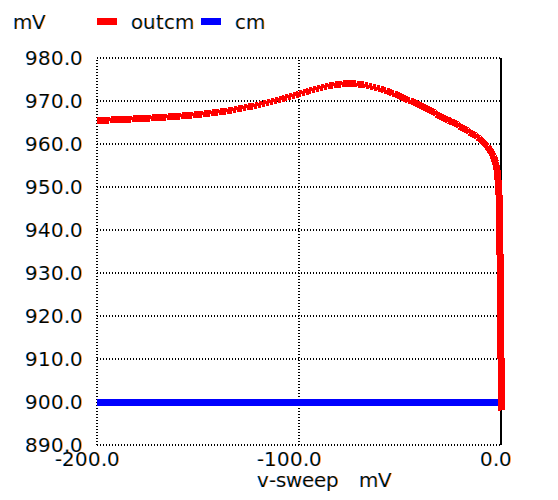
\includegraphics[height=5cm]{3-dc-cm.png}
        \caption{}\label{fig:3-dc-cm}
    \end{minipage}\hfill
    \begin{minipage}{.45\textwidth}
        \centering
        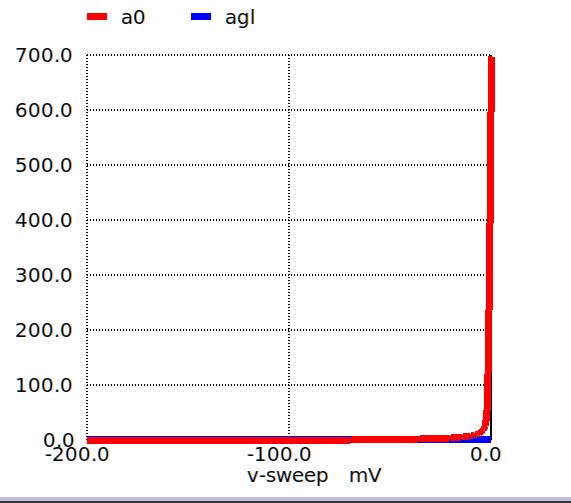
\includegraphics[height=5cm]{3-dc-a.png}
        \caption{}\label{fig:3-dc-a}
    \end{minipage}
\end{figure}

\subsubsection{AC Analyse}

Im Frequenzgang ist nocheinmal die erhöhung der Verstärkung und ein hohes CMRR
zu erkennen. Jedoch ist aufgrund der größeren Gäte weiten und Längen die Kapazität
gestiegen, welche die Bandbreite einschränkt. Bereits im Kilohertz Bereich
fängt die Verstärkung an stark abzufallen.

\begin{figure}[h]
\begin{minipage}{.32\textwidth}
    \centering
    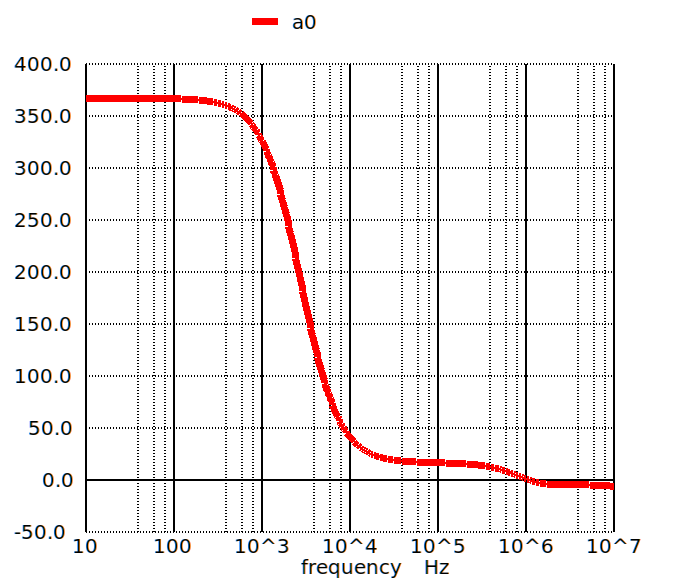
\includegraphics[width=\textwidth]{3-ac-a0.png}
\end{minipage}\hfill
\begin{minipage}{.32\textwidth}
    \centering
    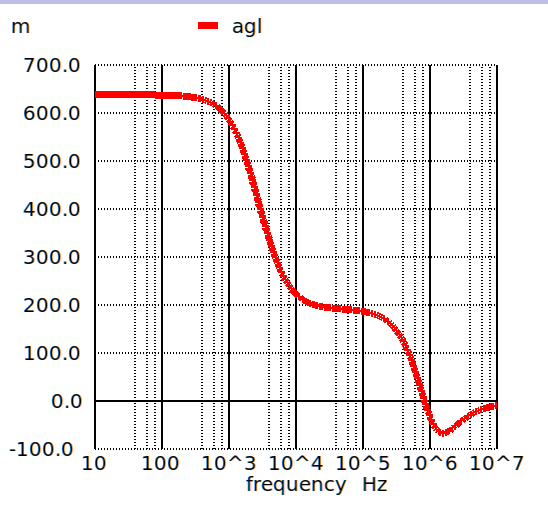
\includegraphics[width=\textwidth]{3-ac-agl.png}
\end{minipage}\hfill
\begin{minipage}{.32\textwidth}
    \centering
    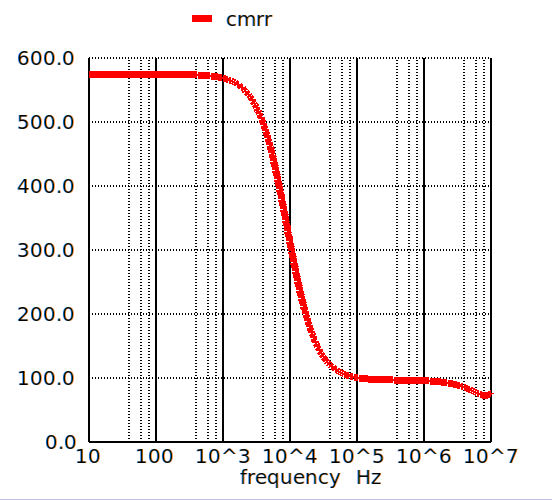
\includegraphics[width=\textwidth]{3-ac-cmrr.png}
\end{minipage}
\end{figure}


%% 
%%%%%%%%%%%%%%%%%%%%%%%%%%%%%%%%%%%%%%%%%%%%%%%%%%%%%%%%%%%%%%%%%%%%%%%%%%%%%%%%

\end{document}
\endinput
